% !TeX root = slides.tex
\documentclass[aspectratio=169,12pt]{beamer}
\usetheme{metropolis}
\usepackage{booktabs}
\usepackage{tikz}
\usetikzlibrary{positioning,arrows.meta,fit,backgrounds}
\usepackage{xcolor}
\usepackage{amsmath}
\usepackage{fontspec}
\usepackage{xeCJK}

\setCJKmainfont{Noto Sans CJK TC}
\setCJKsansfont{Noto Sans CJK TC}

\definecolor{good}{HTML}{2E7D32}
\definecolor{bad}{HTML}{C62828}
\definecolor{neutral}{HTML}{1565C0}
\definecolor{highlight}{HTML}{E65100}

\title{Token-Level GFMs for Metagenomic Classification}
\subtitle{Progress, Findings, and Publication Plan}
\author{Yu-Ming Jen}
\institute{NTU CSIE}
\date{May 2026}

% -----------------------------------------------------------------------
\begin{document}

\maketitle

% -----------------------------------------------------------------------
\begin{frame}{研究問題 Research Questions}
\begin{columns}
\column{0.5\textwidth}
\textbf{Q1: Token-level vs.\ mean-pool}\\[4pt]
保留完整 token 序列（attention-pool + LoRA）是否比 frozen mean-pool 更好？

\vspace{1em}
\textbf{Q2: Pre-training vs.\ Tokenization}\\[4pt]
GFM 大規模預訓練能否彌補 6-mer tokenization 對長程 $k$-mer 判別力的限制？

\column{0.5\textwidth}
\begin{block}{Short Answer}
\textbf{Q1} Yes: $+13.37$~pp at 5M reads\\[2pt]
\textbf{Q2} No: MT 13-mer \emph{from scratch} beats NT-v2 + LoRA by $\mathbf{+20.35}$~pp
\end{block}
\end{columns}
\end{frame}

% -----------------------------------------------------------------------
\begin{frame}{Experiment Map — All Experiments Completed}
\centering
\resizebox{\textwidth}{!}{%
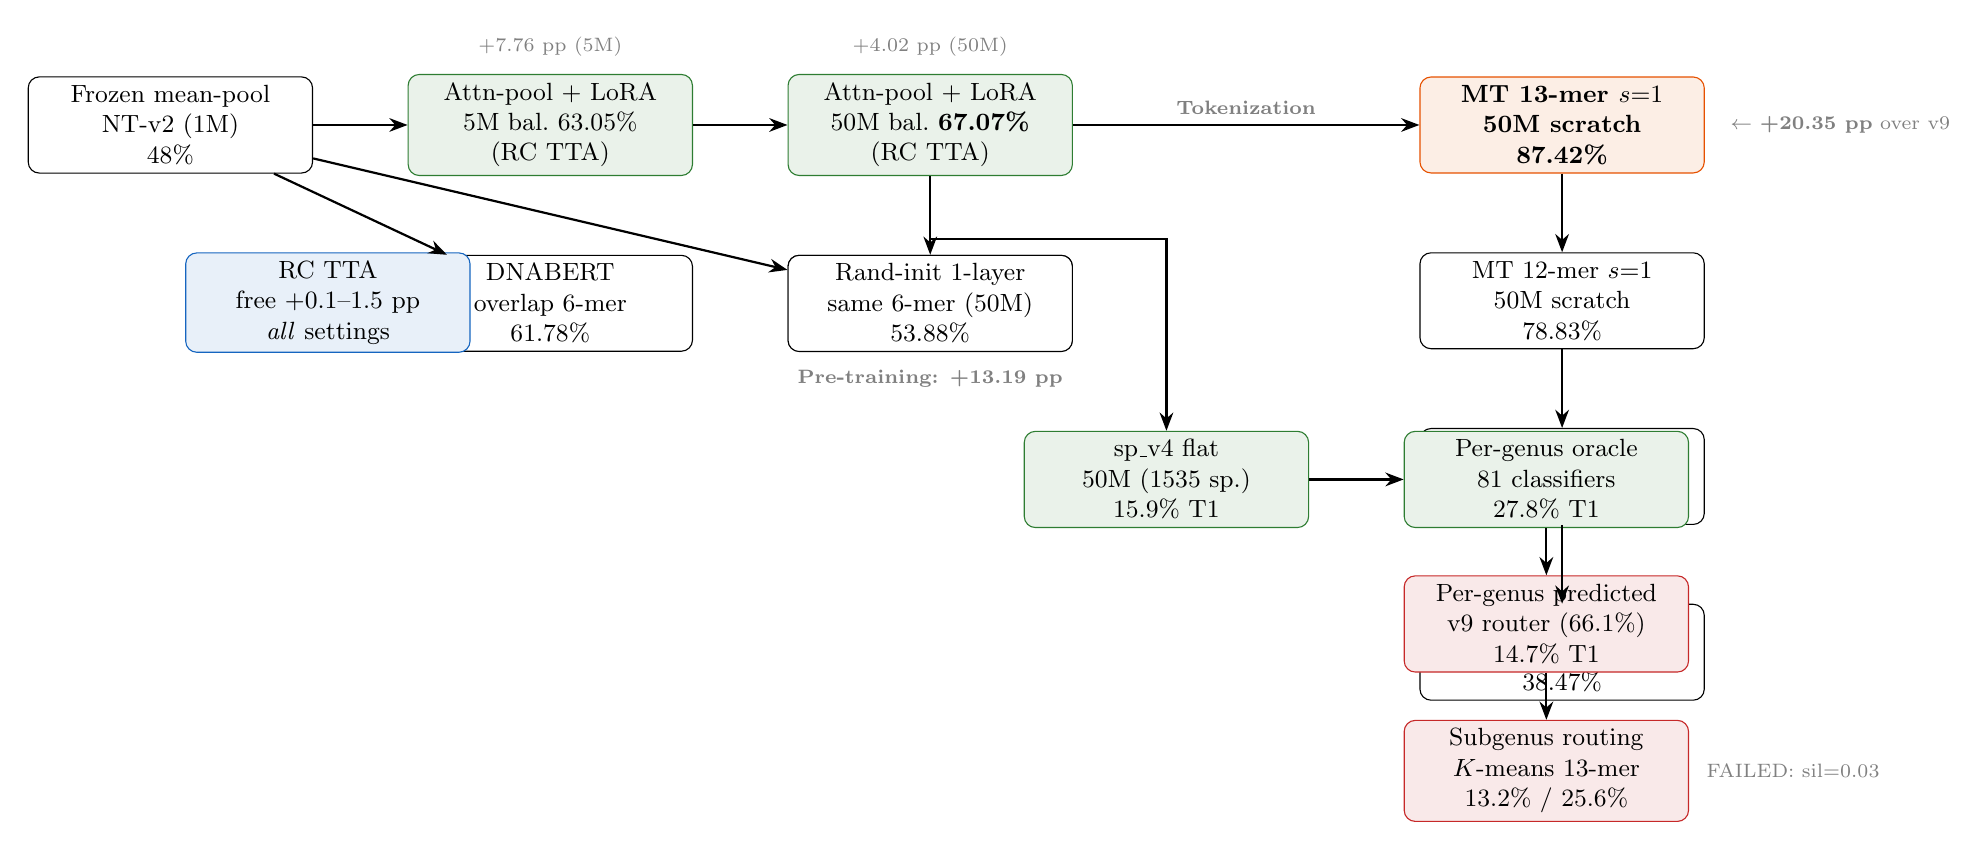
\begin{tikzpicture}[
  node distance = 6mm and 12mm,
  box/.style  = {draw, rounded corners, fill=white, text width=34mm,
                 align=center, font=\small, inner sep=3pt},
  good/.style = {box, draw=good,  fill=good!10},
  bad/.style  = {box, draw=bad,   fill=bad!10},
  pivot/.style= {box, draw=highlight, fill=highlight!10, font=\small\bfseries},
  arrow/.style= {-Stealth, thick},
  label/.style= {font=\scriptsize, text=gray}
]

% ---- Baseline ----
\node[box] (base) {Frozen mean-pool\\NT-v2 (1M)\\48\%};

% ---- Token-level arm ----
\node[good, right=of base]  (v8)   {Attn-pool + LoRA\\5M bal.\ 63.05\%\\(RC TTA)};
\node[good, right=of v8]    (v9)   {Attn-pool + LoRA\\50M bal.\ \textbf{67.07\%}\\(RC TTA) \checkmark};

% ---- Scaling annotations ----
\node[label, above=1mm of v8] {+7.76 pp (5M)};
\node[label, above=1mm of v9] {+4.02 pp (50M)};

% ---- GFM comparison (5M) ----
\node[box, below=10mm of v8] (dna1) {DNABERT\\overlap 6-mer\\61.78\%};
\node[box, right=of dna1]    (dna2) {DNABERT-2\\BPE 117M\\58.88\%};

% ---- Backbone ablation (50M) ----
\node[box, below=10mm of v9] (v11) {Rand-init 1-layer\\same 6-mer (50M)\\53.88\%};
\node[label, below=1mm of v11] {\textbf{Pre-training: +13.19 pp}};

% ---- Tokenization arm (MT) ----
\node[pivot, right=44mm of v9] (mt13) {MT 13-mer $s{=}1$\\50M scratch\\\textbf{87.42\%} \checkmark};
\node[box, below=10mm of mt13] (mt12) {MT 12-mer $s{=}1$\\50M scratch\\78.83\%};
\node[box, below=10mm of mt12] (mt6o) {MT 6-mer $s{=}1$\\50M scratch\\48.87\%};
\node[box, below=10mm of mt6o] (mt6n) {MT 6-mer $s{=}6$\\50M scratch\\38.47\%};

\node[label, right=2mm of mt13] {$\leftarrow$ \textbf{+20.35 pp} over v9};

% ---- Species arm ----
\node[good, below=10mm of v11, xshift=30mm] (spv4) {sp\_v4 flat\\50M (1535 sp.)\\15.9\% T1 \checkmark};
\node[good, right=of spv4]  (pgora) {Per-genus oracle\\81 classifiers\\27.8\% T1 \checkmark};
\node[bad,  below=6mm of pgora] (pgpred) {Per-genus predicted\\v9 router (66.1\%)\\14.7\% T1};
\node[bad,  below=6mm of pgpred] (subg)  {Subgenus routing\\$K$-means 13-mer\\13.2\% / 25.6\%};
\node[label, right=1mm of subg] {FAILED: sil=0.03};

% ---- RC TTA note ----
\node[box, draw=neutral, fill=neutral!10, below=10mm of base, xshift=20mm]
    (rctta) {RC TTA\\free +0.1–1.5 pp\\\emph{all} settings};

% ---- Arrows ----
\draw[arrow] (base)  -- (v8);
\draw[arrow] (v8)    -- (v9);
\draw[arrow] (base)  -- (dna1);
\draw[arrow] (base)  -- (dna2);
\draw[arrow] (v9.south) -- ++(0,-5mm) -| (v11.north);
\draw[arrow] (v9)    -- node[above, label]{\textbf{Tokenization}} (mt13);
\draw[arrow] (v9.south) -- ++(0,-8mm) -| (spv4.north);
\draw[arrow] (spv4)  -- (pgora);
\draw[arrow] (pgora) -- (pgpred);
\draw[arrow] (pgpred)-- (subg);
\draw[arrow] (mt13)  -- (mt12);
\draw[arrow] (mt12)  -- (mt6o);
\draw[arrow] (mt6o)  -- (mt6n);

\end{tikzpicture}%
}
\end{frame}

% -----------------------------------------------------------------------
\begin{frame}{Finding 1 — Data Scaling Within NT-v2}
\begin{columns}
\column{0.55\textwidth}
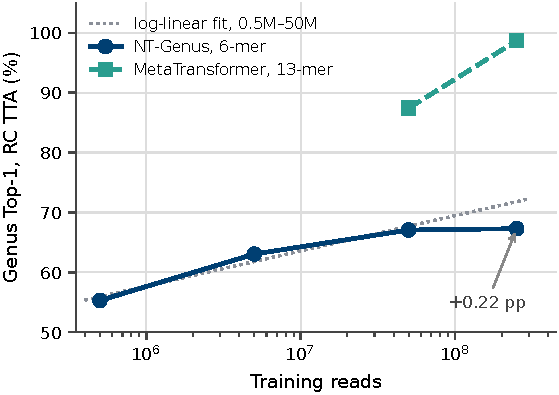
\includegraphics[width=\linewidth]{../figures/data_scaling.pdf}

\column{0.45\textwidth}
\begin{block}{結論}
\begin{itemize}
  \item $500\text{K}\!\to\!5\text{M}$: $+7.76$~pp
  \item $5\text{M}\!\to\!50\text{M}$: $+4.02$~pp
  \item Diminishing returns 明顯
  \item 架構 / 訓練技巧: $\leq\!\pm0.5$~pp
\end{itemize}
\end{block}

\vspace{4pt}
{\small \textbf{在 NT-v2 框架內，資料量是唯一重要的變因}}
\end{columns}
\end{frame}

% -----------------------------------------------------------------------
\begin{frame}{Finding 2 — Pre-Training Advantage (Fixed Tokenization)}
\begin{columns}
\column{0.55\textwidth}
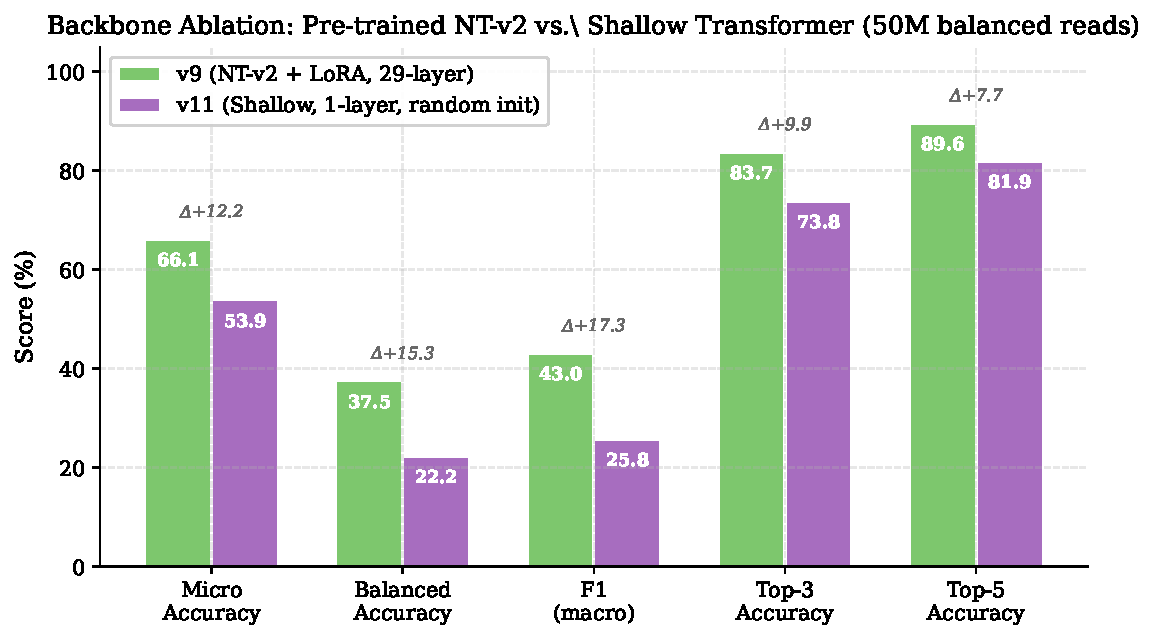
\includegraphics[width=\linewidth]{../figures/backbone_ablation.pdf}

\column{0.45\textwidth}
\begin{tabular}{lc}
\toprule
Model & Acc (RC TTA) \\ \midrule
NT-v2 pre-trained & \textbf{67.07\%} \\
Rand-init 1-layer & 53.88\% \\
\midrule
\textbf{Gap} & \textbf{+13.19 pp} \\
\bottomrule
\end{tabular}

\vspace{8pt}
{\small 相同 tokenization、相同 50M 資料 → pre-training 有實質貢獻}
\end{columns}
\end{frame}

% -----------------------------------------------------------------------
\begin{frame}{Finding 3 — Tokenization Dominates (Key Finding)}
\centering
\begin{tabular}{lllc}
\toprule
\textbf{Model} & \textbf{Tokenization} & \textbf{Pre-trained?} & \textbf{Genus Top-1} \\
\midrule
MT 6-mer $s=6$   & non-overlap & No  & 38.47\% \\
MT 6-mer $s=1$   & overlap     & No  & 48.87\% \\
NT-v2 + LoRA     & non-overlap & \textbf{Yes (498M)} & 67.07\% \\
MT 12-mer $s=1$  & overlap     & No  & 78.83\% \\
\rowcolor{highlight!20}
MT 13-mer $s=1$  & overlap     & No  & \textbf{87.42\%} \\
\bottomrule
\end{tabular}

\vspace{10pt}
\large $\Delta = +20.35$~pp: MT 13-mer scratch \textbf{vs.} NT-v2 + LoRA\\[4pt]
\normalsize NT-v2 的 non-overlapping 6-mer tokenizer 是主要結構性瓶頸
\end{frame}

% -----------------------------------------------------------------------
\begin{frame}{Finding 4 — Hierarchical Pipeline \& Subgenus Routing}
\begin{columns}
\column{0.5\textwidth}
\textbf{Hierarchical results (independent 100K test)}\\[6pt]
\begin{tabular}{lc}
\toprule
Mode & Sp.\ Top-1 \\
\midrule
sp\_v4 flat baseline       & 15.9\% \\
sp\_v4 oracle genus        & 27.4\% \\
Per-genus \textbf{oracle}  & \textbf{27.8\%} \\
Per-genus predicted (v9)   & 14.7\% \\
\midrule
Subgenus hard routing      & 13.2\% \\
Subgenus soft routing      & 13.6\% \\
\bottomrule
\end{tabular}

\column{0.5\textwidth}
\begin{alertblock}{Subgenus Routing: FAILED}
\begin{itemize}
  \item Collinsella silhouette $= 0.03$
  \item UMAP: continuous blob，無法分群
  \item 加入 subgenus tier 反而 $\downarrow$ 1.5~pp
\end{itemize}
\end{alertblock}

\vspace{6pt}
\begin{block}{Root Cause}
NT-v2 的 6-mer embedding 無法區分同屬物種 → 問題在表示層，不在路由深度
\end{block}
\end{columns}
\end{frame}

% -----------------------------------------------------------------------
\begin{frame}{Finding 5 — Sample-Level Utility}
\begin{columns}
\column{0.48\textwidth}
\textbf{Relative Abundance (100 samples)}\\[4pt]
\begin{tabular}{lcc}
\toprule
Metric & NT-v2 & MT 13 \\
\midrule
Pearson $r$  & 0.993 & 0.999 \\
Bray-Curtis  & 0.094 & 0.028 \\
\bottomrule
\end{tabular}

\vspace{8pt}
\textbf{Binary Detection (200 samples)}\\[4pt]
\begin{tabular}{lcc}
\toprule
Metric & NT-v2 & MT 13 \\
\midrule
ROC AUC          & 0.705 & 0.900 \\
Sens @ 95\% spec & 17.2\% & 47.7\% \\
\bottomrule
\end{tabular}

\column{0.52\textwidth}
\begin{block}{結論}
\begin{itemize}
  \item 67\% 單讀準確度 → $r=0.993$ 豐度估計
  \item $\geq\!1\%$ 豐度 100\% 偵測靈敏度
  \item Binary detection 受限於 0.28\% noise floor
  \item 提升 per-read acc 對 binary detection 有非線性幫助
\end{itemize}
\end{block}
\end{alertblock}{\small 注意: 評估在固定群落組成下，非真實多樣性社群}
\end{columns}
\end{frame}

% -----------------------------------------------------------------------
\begin{frame}{故事完整性 — The Thesis Has a Complete Arc}
\begin{tikzpicture}[node distance=8mm,
  step/.style={draw, rounded corners, fill=neutral!10, text width=38mm,
               align=center, font=\small, inner sep=4pt}]
\node[step] (s1) {資料量是 NT-v2 框架內\\主要因素\\(500K→50M)};
\node[step, right=of s1] (s2) {Pre-training 有效\\固定tokenization下\\+13.19 pp};
\node[step, right=of s2] (s3) {Tokenization\\跨架構最重要\\+20.35 pp};
\node[step, right=of s3] (s4) {Hierarchical validated;\\subgenus routing failed\\→ 表示層瓶頸確認};

\draw[-Stealth,thick] (s1) -- (s2);
\draw[-Stealth,thick] (s2) -- (s3);
\draw[-Stealth,thick] (s3) -- (s4);

\node[draw=good, fill=good!10, rounded corners, below=12mm of s2, text width=80mm,
      align=center, font=\small]
    {結論：NT-v2 的 non-overlapping 6-mer tokenizer 是唯一瓶頸\\
     解法：以 overlapping 13-mer 預訓練的微生物基礎模型};
\end{tikzpicture}

\vspace{4pt}
{\small 每一步都有受控實驗（固定其他變因）支持，構成 falsifiable scientific argument}
\end{frame}

% -----------------------------------------------------------------------
\begin{frame}{為什麼現在可以收工？}
\begin{columns}
\column{0.48\textwidth}
\textbf{已完成 (Done)}
\begin{itemize}
  \item[$\checkmark$] 全部 controlled ablation
  \item[$\checkmark$] Data scaling 500K–50M
  \item[$\checkmark$] RC TTA analysis
  \item[$\checkmark$] GFM cross-architecture comparison
  \item[$\checkmark$] Hierarchical pipeline (per-genus oracle)
  \item[$\checkmark$] Subgenus routing (negative)
  \item[$\checkmark$] Sample-level evaluation
  \item[$\checkmark$] Thesis draft 完成
\end{itemize}

\column{0.52\textwidth}
\textbf{若繼續做的邊際貢獻}
\begin{itemize}
  \item[$\to$] 258M 完整訓練:\\NT-v2 框架內最多再+5pp\\不改變任何結論
  \item[$\to$] Pre-train 13-mer GFM:\\6–12個月 + GTDB 400K genomes\\這是全新 project
  \item[$\to$] Real microbiome validation:\\需要合作夥伴、真實樣本
\end{itemize}

\vspace{6pt}
\begin{alertblock}{機會成本}
每多等一個月 = 競爭風險 + 未發表
\end{alertblock}
\end{columns}
\end{frame}

% -----------------------------------------------------------------------
\begin{frame}{未來方向 — 必須決定的三條路}
\centering
\begin{tikzpicture}[
  route/.style={draw, rounded corners, text width=42mm, align=center,
                font=\small, inner sep=5pt},
  now/.style={route, fill=good!15, draw=good},
  mid/.style={route, fill=neutral!15, draw=neutral},
  long/.style={route, fill=gray!15, draw=gray}
]
\node[now]  (p1) at (0,0)
    {\textbf{方向 A: 發表現有結果}\\[4pt]
     Briefings in Bioinformatics\\NAR Genomics \& Bioinformatics\\[4pt]
     \textcolor{good}{時間: 3–4 個月}\\
     \textcolor{good}{難度: 低（thesis → paper）}};

\node[mid]  (p2) at (5.5,0)
    {\textbf{方向 B: 258M 完整訓練}\\[4pt]
     NT-v2 框架延伸\\預期 ~75\% genus acc\\[4pt]
     \textcolor{neutral}{時間: +2 個月}\\
     \textcolor{neutral}{不改變結論}};

\node[long] (p3) at (11,0)
    {\textbf{方向 C: 新 GFM 預訓練}\\[4pt]
     GTDB + 13-mer overlapping\\預期 >90\% genus acc\\[4pt]
     \textcolor{gray}{時間: 6–12+ 個月}\\
     \textcolor{gray}{全新 project}};

\node[above=3mm of p1, font=\small\bfseries, text=good]  {$\Rightarrow$ 建議立即啟動};
\node[above=3mm of p2, font=\small\bfseries, text=neutral] {$\Rightarrow$ 可平行};
\node[above=3mm of p3, font=\small\bfseries, text=gray]  {$\Rightarrow$ 下一個 project};
\end{tikzpicture}
\end{frame}

% -----------------------------------------------------------------------
\begin{frame}{建議投稿期刊 \& Timeline}
\begin{columns}
\column{0.5\textwidth}
\textbf{Target Venues}\\[6pt]
\begin{tabular}{ll}
\toprule
Venue & Type \\ \midrule
\textit{Briefings in Bioinformatics} & Journal (IF~9.5) \\
\textit{NAR Genomics \& Bioinformatics} & Journal (OA) \\
\textit{Bioinformatics} (OUP) & Journal \\
ISMB 2027 & Conference \\
\bottomrule
\end{tabular}

\vspace{8pt}
\textbf{Paper的主要 novelty}
\begin{itemize}\small
  \item First systematic GFM ablation for metagenomics
  \item Tokenization $\gg$ pre-training (controlled experiment)
  \item Hierarchical pipeline + negative subgenus result
\end{itemize}

\column{0.5\textwidth}
\textbf{Proposed Timeline}\\[6pt]
\begin{tabular}{ll}
\toprule
Month & Milestone \\ \midrule
May   & 論文口試通過 \\
Jun   & Paper draft v1 \\
Jul   & Internal review \\
Aug   & Submit to BIB/NAR \\
      & (258M 平行訓練) \\
Oct   & Revision round 1 \\
\bottomrule
\end{tabular}
\end{columns}
\end{frame}

% -----------------------------------------------------------------------
\begin{frame}{Summary}
\begin{block}{What We Found}
\begin{enumerate}
  \item Data volume $\gg$ training tricks within NT-v2
  \item Pre-training $+13.19$~pp (fixed 6-mer tokenization)
  \item Tokenization design $+20.35$~pp (cross-architecture)
  \item Hierarchical decomposition correct direction; subgenus routing fails due to representation bottleneck
  \item 67\% per-read acc $\to$ $r=0.993$ abundance estimation at sample level
\end{enumerate}
\end{block}

\begin{alertblock}{Bottom Line}
NT-v2 的瓶頸是 6-mer tokenizer，不是 backbone 大小或 LoRA 策略。\\
下一步是預訓練 overlapping 13-mer 的微生物 GFM，這是一個獨立 project。\\
\textbf{現在的結果已足夠發表一篇完整論文。}
\end{alertblock}
\end{frame}

% -----------------------------------------------------------------------
\end{document}
